\documentclass[12pt,oneside,a4paper]{article}
\usepackage{tabularx}
\usepackage{graphicx}
\usepackage[hidelinks]{hyperref}
\usepackage[top=1.2in]{geometry}
\usepackage{abstract}
\usepackage{setspace}
\usepackage{enumitem}
\usepackage[nodayofweek]{datetime}
\usepackage{cite}

\usepackage{lipsum}
\usepackage{xcolor}

\newcommand\todo[1]{\textcolor{blue}{#1}}
\newcommand\placeholder[1]{\todo{\lipsum[#1]}}

\providecommand\phantomsection{}

\tolerance=1
\emergencystretch=\maxdimen
\hyphenpenalty=10000
\hbadness=10000

\renewcommand{\abstractnamefont}{\normalfont\Large\bfseries}

\title{{\huge\textbf{Ramaiah Institute of Technology}} \\
	\small{(An Autonomous Institute, Affiliated to VTU)} \\ [10pt]
	MSR Nagar, MSRIT post, Bangalore - 54 \\ [25pt]
	A Dissertation PBL Report on \\ [10pt]
	{\Large \textbf{Sign Language Recognition}} \\ [20pt]
	Submitted by \\ [25pt]
	\begin{minipage}{0.6\textwidth}
		M Sneha \hfill 1MS14CS058 \\
		Mipsa Patel \hfill 1MS14CS148 \\
		Tilak S Naik \hfill 1MS14CS134 \\
		Vibha Karanth \hfill 1MS14CS136
	\end{minipage} \\ [30pt]
	\textit{\textbf{Bachelor of Engineering in Computer Science \& Engineering}} \\ [10pt]
	Under the guidance of \\ [20pt]
	\begin{minipage}{0.4\textwidth}
		\centering
		Pramod Sunagar \\
		Assistant Professor \\
		Department of Computer Science \\
		Ramaiah Institute of Technology
	\end{minipage} \\ [10pt]
	
\includegraphics{rit.png} \\ [20pt]
	\textbf{DEPARTMENT OF COMPUTER SCIENCE \& ENGINEERING} \\ [20pt]
	\textbf{M. S. RAMAIAH INSTITUTE OF TECHNOLOGY} \\
	\textbf{(Autonomous Institute, Affiliated to VTU)} \\
	\textbf{BANGALORE - 560054} \\
	\textbf{\href{www.msrit.edu}{www.msrit.edu}, 2017}
}

\author{}
\date{}

\begin{document}
	\maketitle
	\thispagestyle{empty}

	\newpage
	\pagenumbering{roman}

	\section*{\centering{\uppercase{Declaration}}}
		\addcontentsline{toc}{section}{Declaration}
		I Student of seventh semester BE, Dept of Computer Science and Engineering, Ramaiah Institute of Technology, Bangalore, hereby declare that the project entitled ``Sign Language Recognition", thesis completed and written by me under the guidance of Pramod Sunagar, Dept of CSE, Bangalore for the partial fulfillment of the requirements for the award of the degree of Bachelor of Engineering. \\ [80pt]
		Place: Bangalore \\
		Date: \formatdate{28}{10}{2017} \\ [20pt]
		(1MS14CS058 M Sneha) \\
		(1MS14CS148 Mipsa Patel) \\
		(1MS14CS134 Tilak S Naik) \\
		(1MS14CS136 Vibha Karanth) \\
	\newpage

	\section*{\centering{\uppercase{Acknowledgement}}}
		\addcontentsline{toc}{section}{Acknowledgement}
		First and foremost, my utmost gratitude to Pramod Sunagar, Dept of CSE, MSRIT whose sincerity and encouragement we will never forget. He has been our inspiration as we overcame all the obstacles in the completion of this project work. \\
		\\
		Dr. Anita Kanavalli, Head of the Department of Computer Science and Engineering, had kind concern and consideration regarding project work and we would like to thank her for continuous support. \\
		\\
		We would like to thank our beloved principal Dr. N. V. R. Naidu for his support and encouragement. \\
		\\
		This work would not have been possible without the guidance and help of several individuals who in one way or another contributed their valuable assistance in preparation and completion of this study. \\
		\\
		We would like to express sincere thanks to all the teaching and non-teaching faculty of CSE Department and my dear friends who helped in all the ways while preparing the report.
	\newpage

	\null
	\vspace{\fill}

	\phantomsection
	\addcontentsline{toc}{section}{Abstract}
	\begin{abstract}
		\normalsize
		\doublespacing
		Sign language is the language used by the hearing and speech impaired to communicate among themselves and others. Unless the concerned people know the sign language properly, there is a communication barrier between them. In most cases, an interpreter is required to carry out such a conversation. To reduce the dependency of the hearing and speech impaired people on interpreters, we develop a real time sign language detection system that converts the gestures from images and videos into English sentences, using various deep learning techniques.
	\end{abstract}

	\vspace{\fill}
	\null
	\newpage

	\tableofcontents

	\newpage
	\pagenumbering{arabic}

	\section{Introduction}

		\subsection{General Introduction}
			Sign Language is a vision based language that uses the movements of the hands and facial expressions for communication. Subtle differences among different hand gestures can have a huge impact on the meaning that they convey. Along with this, it is important to prevent the background noise of the image from affecting the gestures being communicated. We consider such problems and challenges and develop an effective sign language recognition system.

		\subsection{Statement of the Problem}
			There exist models that convert American Sign Language to sentences. However, most of these techniques are not based on deep learning. These models also cannot handle the nuances of the Indian Sign Language. We use the Indian sign Language and deep neural networks to develop a model that can convert gestures of ISL into English text.

		\subsection{Objectives of the project}

			\begin{itemize}
				\item To develop an Indian Sign Language recognition system.
				\item To design a deep neural network which can give a better performance and robustness compared to the existing image processing and machine learning models.
			\end{itemize}

		\subsection{Project deliverables}
		
			\begin{itemize}
				\item An application that obtains frames from sign language communication videos, processes them, and obtains the meaning being conveyed by them in the form of English text.
				\item Comparison of performance of our model with existing algorithms used for sign language recognition.
			\end{itemize}

		\subsection{Current Scope}
			    Image and video processing is one of the important fields in Machine Learning and Deep Learning right now. The huge number of images and videos on social media and otherwise has led to an increased interest in the field. The algorithms and techniques developed as a result of this can be used in more impactful fields like helping the speech and hearing impaired lead more convenient lives. \\
			\\
			The hand signs along with the emotions displayed by the individual provide the content and tone of the sentence. A tool to convert their words into a widely used language enhances their ability to communicate.

		\subsection{Future Scope}
			Since such applications will always be necessary, research and development of new algorithms to improve the efficiency of interpretation of sign language will be endless. Deep learning has a lot more to offer than what has already been explored. With such possibilities, there will always be scope to develop newer models that can be used in sign language recognition. The models used in this can also be used in other applications such as gesture controlled systems, tracking unusual activity, etc. with slight tweaks. With slight modification, it can also be used for recognition of other sign languages. \\
			\\
			Moreover, the current work can be further extended to output speech instead of text. A similar generative model can be used to map speech or text to actions by stitching together pre-recorded videos or actually generate an interface with a skeletal structure. This model can be seamlessly integrated with various applications on different platforms to support high productivity.


	\section{Literature Survey}

		\subsection{Introduction}
			There have been a lot of different approaches used to solve the problem of sign language recognition. However, most of these use image processing in MATLAB, upon which Machine Learning algorithms are applied. There has also been some work done using artificial neural networks.

		\subsection{Related work with the citation of references}
			\cite{dutta:2015} deals with the double handed Indian Sign Language. It is captured as a series of images, processed with the help of MATLAB and then converted to speech and text. However this approach uses image processing techniques which are highly sensitive to lighting conditions. \\
			\\
			\cite{DK:2014} proposes an image processing, computer vision and neural network based approach to identify the characteristics of the hand in images taken from a video through webcam. Identification of hand shapes from continuous frames is done by using series of image processing operations. Interpretation of signs and corresponding meaning is identified by using Haar Cascade Classifier. Finally displayed text is converted into speech using speech synthesizer. \\
			\\
			\cite{autoisl:2013} proposes a system that consists of three phases, a training phase, a testing phase and a recognition phase. In the training phase, each class is trained with a multiclass support vector machine (MSVM). Hu invariant moment and structural shape descriptors are combined to make a combinational feature vector that are to be extracted from the input image in the testing phase after applying preprocessing. In the recognition phase, different classes are used for testing an input gesture.

		\subsection{Conclusion of Survey}
			Deep neural networks have revolutionized how different Machine Learning problems are approached. Using them to solve this problem can give significant results, and that is precisely what this project explores.

	\section{Project Management Plan}

		\subsection{Schedule of the project}
			\placeholder{2}

	\section{Software Requirement Specification}

		\subsection{Project Overview}
			Images of numbers and letters, and videos of words and sentences are fed as input to the model and interpreted text is received as output using various deep learning techniques.

		\subsection{Hardware}
			We use a system with NVIDIA\textsuperscript{\textregistered} GeForce\textsuperscript{\textregistered} 940MX (4 GB DDR3) GPU and 8 GB RAM to perform our experiment. A camera is required to record hand gestures and facial expressions.

		\subsection{Software Requirements}

			\begin{itemize}
				\item Python
				\item OpenCV
				\item CUDA
				\item PyTorch for training and testing the deep neural network.
			\end{itemize}

		\subsection{Functional Requirements}

			\begin{itemize}
				\item Take image and video inputs of sign language conversation.
				\item Extract frames from videos for training.
				\item A training algorithm to reduce train-test error and generalize the model to make it invariant to lighting conditions.
				\item Convert the received output classes to letters, words or sentences.
			\end{itemize}

	\section{Design}

		\subsection{Introduction}
			This project has been designed such that it incorporates some of the major applications of machine learning and deep learning. Various concepts such as image and video processing, different neural network architectures, etc. are used. Simplicity and effectiveness are the key factors considered while designing and developing this application.

		\subsection{Architecture Design}

			\begin{figure}[htp]
				\centering
				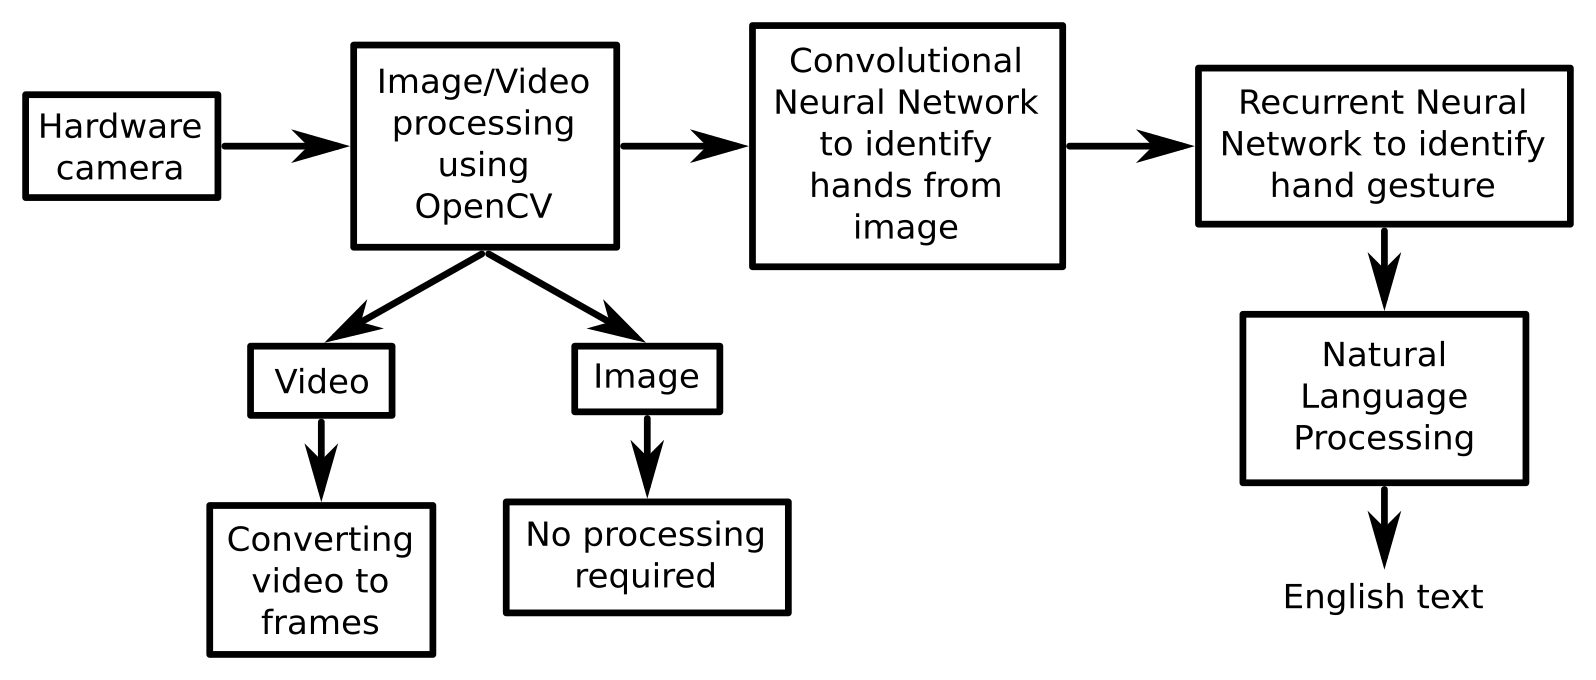
\includegraphics{architecture.png}
				\caption{Architecture}
				\label{fig:ad}
			\end{figure}

			\autoref{fig:ad} gives a brief overview of the architecture that the Sign Language Recognition application follows. \\

			\begin{description}[style=nextline]

				\item[Input module] A camera is required to record the entire conversation. Letters and digits can be considered as single frames, whereas words and sentences are recorded as videos.

				\item[Image and Video Processing] Image and video processing is done using Python and OpenCV. Videos are converted into a series of frames to simplify the process of recognizing gestures.

				\item[Convolutional Neural Network] These networks are a class of deep feedforward neural networks that are based on weight sharing. They are commonly used in image and video processing to identify manifolds. In this project, they are used to identify hands from the given frames.

				\item[Recurrent Neural Network] Recurrent Neural Networks are used whenever memory of previous computations is required. It is used to identify the hand gesture by considering the gestures denoted by the current and the previous frames.

				\item[Natural Language Processing] Natural Language Processing is used to convert the output of the Recurrent Neural Network into proper English text.

			\end{description}

		\subsection{Data Flow Diagram}

			\begin{figure}[htp]
				\centering
				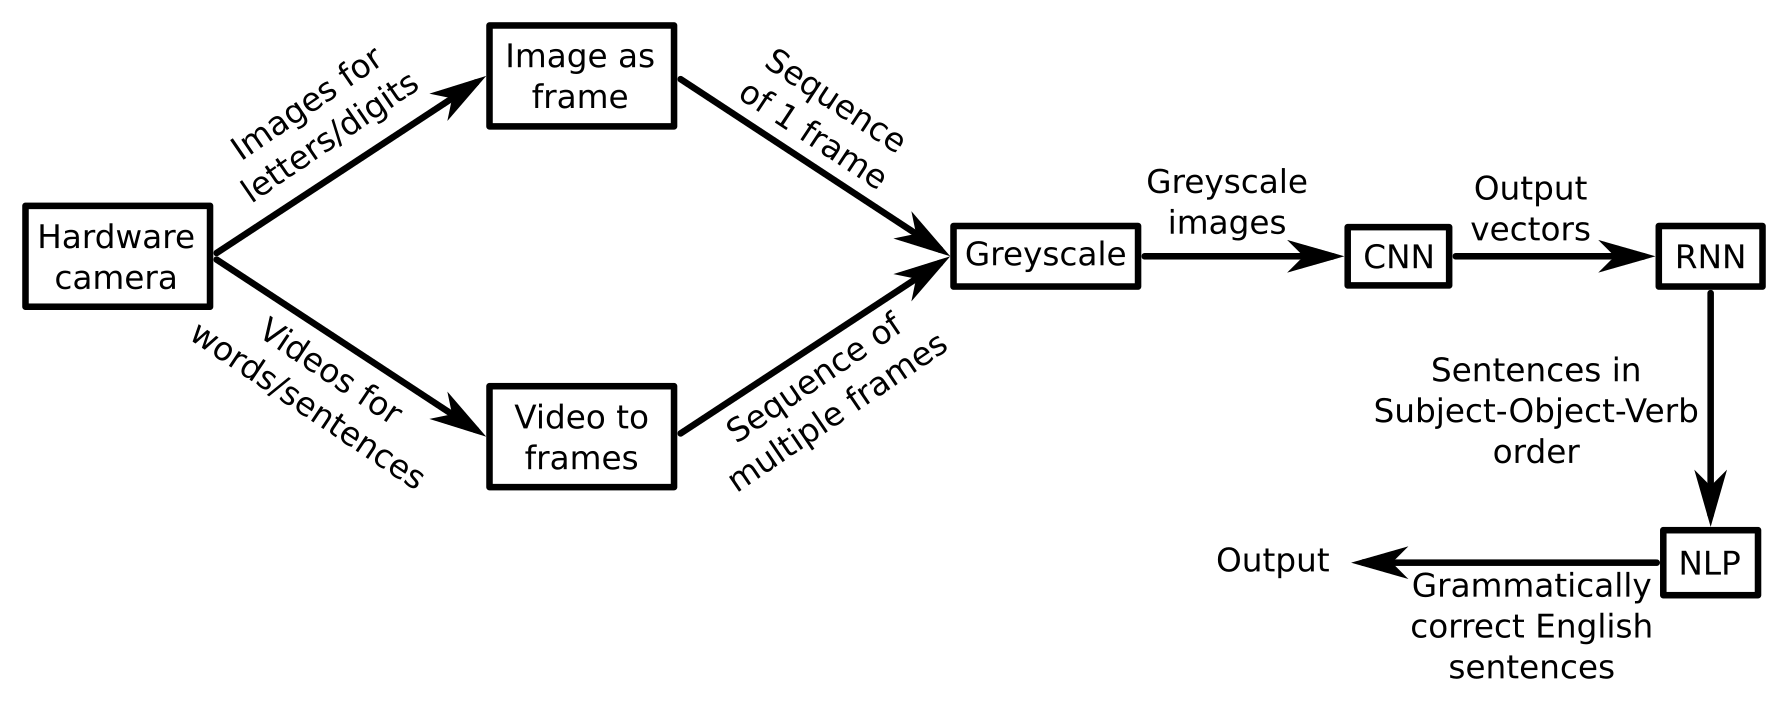
\includegraphics{dfd.png}
				\caption{Data Flow Diagram}
				\label{fig:dfd}
			\end{figure}

			\autoref{fig:dfd} gives the interaction between the different modules of the application and how data flows between them. \\

			\begin{description}[style=nextline]

				\item[Input] The input to the application is taken in the form of either images or videos. Images are considered as sequences of a single frame, whereas videos are converted into a series of frames using OpenCV. \\
				These frames are converted into grayscale images to ensure uniformity in the training and test data in terms of the background, etc.

				\item[Convolutional Neural Network] This neural network is given grayscale images as input. It processes them and converts them to vectors that denote the positions of the hands in the image.

				\item[Recurrent Neural Network] This network takes in the input vectors and outputs letters/digits/words in the order of $subject - object - verb$.

				\item[Natural Language Processing module] NLP is required to convert this sentence in the form of $subject - object - verb$ into a proper English sentence.

			\end{description}

		\subsection{Conclusion}
			It is a challenge to convert hand gestures to text due to wide variety of signs and their associated meanings. It is important that a sign language recognition system is as accurate as possible, due to the number of people that could use it and benefit from it. In such a case, even if such applications already exist, there is always a possibility of developing more effective or advanced systems using newer technology, and the work presented here tests one such approach.

	\bibliographystyle{unsrt}
	\bibliography{report}{}
\end{document}